\documentclass{article}

\usepackage{units} 
\usepackage{graphicx}
\usepackage[fleqn]{amsmath}
\usepackage{cancel}
\usepackage{float}
\usepackage{mdwlist}
\usepackage{booktabs}
\usepackage{cancel}
\usepackage{polynom}
\usepackage{caption}
\usepackage{fullpage}
\usepackage{xfrac}
\usepackage{enumerate}

\newcommand{\degree}{\ensuremath{^\circ}} 
\everymath{\displaystyle}

% \begin{figure}[H]
%   \centering
%   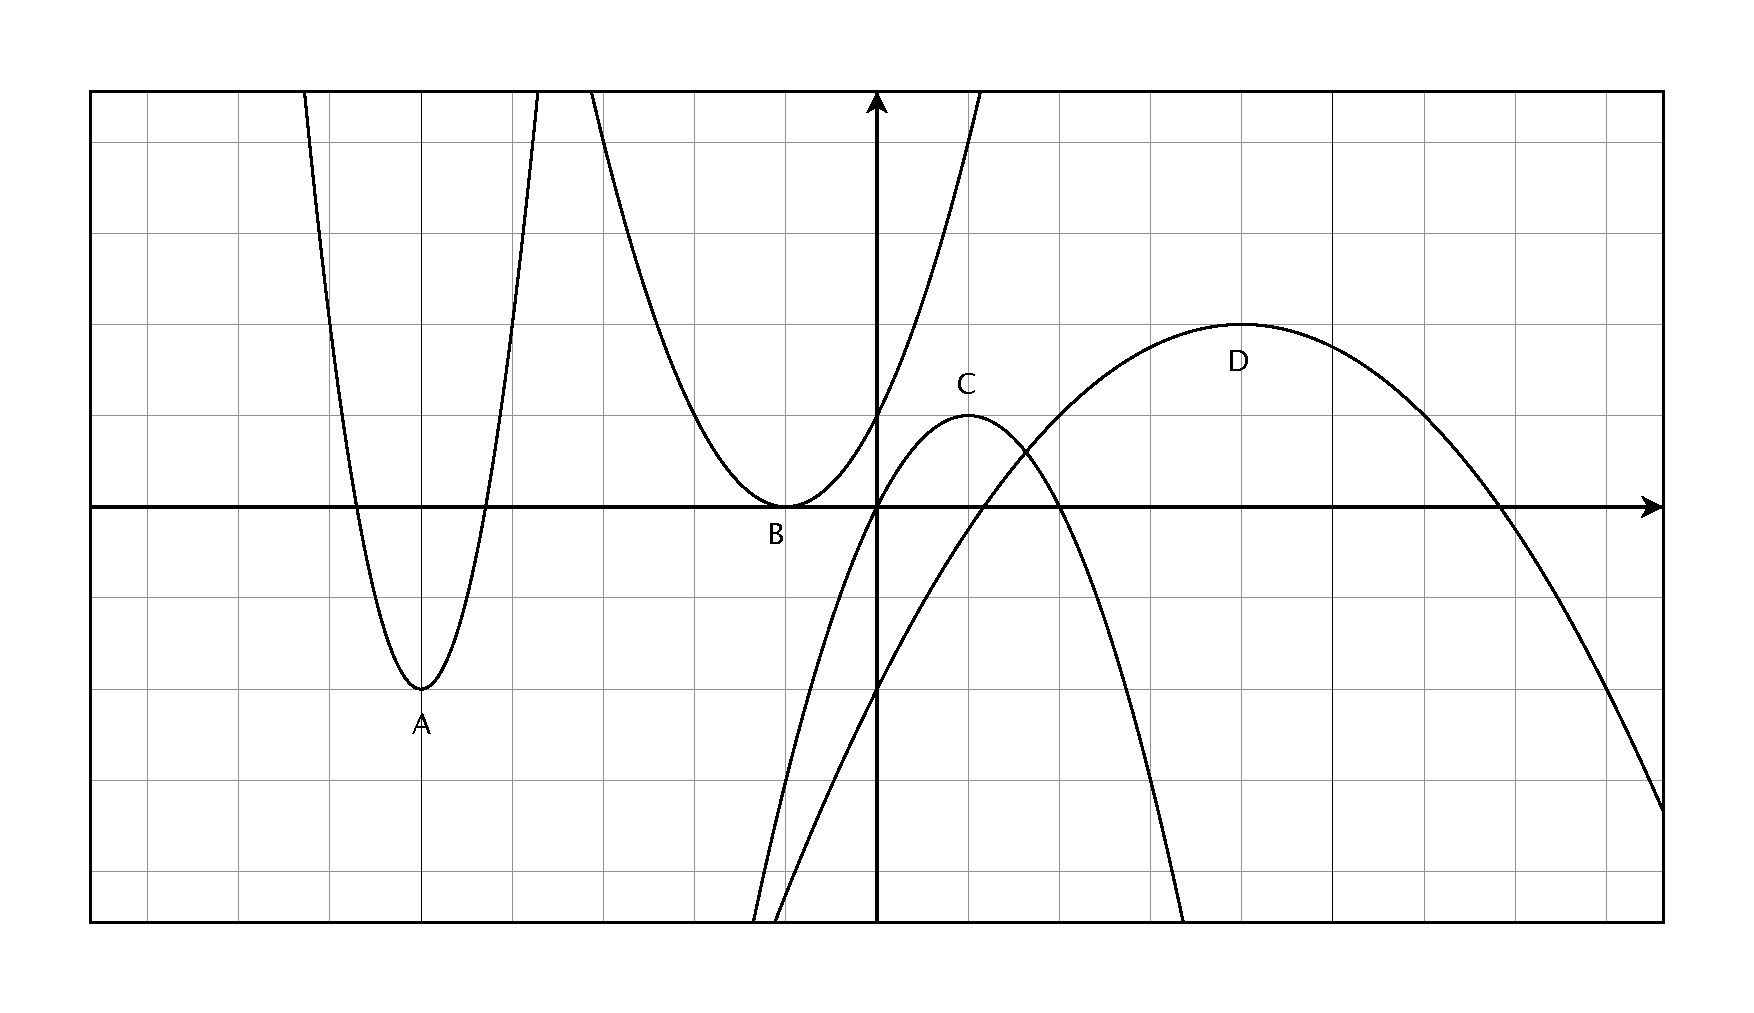
\includegraphics[scale=.3]{problem_7.eps}
%   \caption*{Problem 7}
% \end{figure}

% \begin{tabular}{cc}
% \toprule
% period & amplitude \\
% \midrule
%   $\pi$ & $2$ \\
% \bottomrule
% \end{tabular}

\title{Zooming}
\date{March 27, 2013}

\begin{document}
  \begin{figure}[H]
    \centering
    \includegraphics[scale=0.7]{zoom11.eps}
    \caption*{$f(x) = x^3 - x^2 - 2x$}
  \end{figure}

  \begin{figure}[H]
    \centering
    \includegraphics[scale=0.7]{zoom12.eps}
    \caption*{$f(x) = x^3 - x^2 - 2x$}
  \end{figure}

  \begin{figure}[H]
    \centering
    \includegraphics[scale=0.7]{zoom13.eps}
    \caption*{$f(x) = x^3 - x^2 - 2x$}
  \end{figure}

  \begin{figure}[H]
    \centering
    \includegraphics[scale=0.7]{zoom14.eps}
    \caption*{$f(x) = x^3 - x^2 - 2x$}
  \end{figure}

  \begin{figure}[H]
    \centering
    \includegraphics[scale=0.7]{zoom01.eps}
    \caption*{$f(x) = x^4 + 4x^3 - 13x^2 - 40x + 48$}
  \end{figure}

  \begin{figure}[H]
    \centering
    \includegraphics[scale=0.7]{zoom02.eps}
    \caption*{$f(x) = x^4 + 4x^3 - 13x^2 - 40x + 48$}
  \end{figure}

  \begin{figure}[H]
    \centering
    \includegraphics[scale=0.7]{zoom03.eps}
    \caption*{$f(x) = x^4 + 4x^3 - 13x^2 - 40x + 48$}
  \end{figure}

  \begin{figure}[H]
    \centering
    \includegraphics[scale=0.7]{zoom04.eps}
    \caption*{$f(x) = x^4 + 4x^3 - 13x^2 - 40x + 48$}
  \end{figure}


\end{document}
